\chapter{Revisão Bibliográfica} \label{chap:sota}

\section*{}

Neste capítulo é feita uma revisão bibliográfica e descrito o estado da arte do \emph{software} de localização de falhas, como o \emph{Barinel}, das diferentes abordagens de predição de defeitos e ainda de \emph{Software Repository Mining}.

% Fault Localization Software
\section{\emph{Fault Localization Software}}

O \emph{Fault Localization Software} auxilia na localização automática do código que origina falhas na sua execução, diminuindo o custo desta identificação que teria de ser feita manualmente pelo programador. Existem duas categorias principais: \emph{Spectrum-based diagnosis} e \emph{Model-based diagnosis}.

% 
% ==========
% Program Slicing
% ==========
%

\subsection{\emph{Program Slicing}}

Introduzida por Mark Weiser em 1981 \cite{Weiser1981, Weiser1982}, esta técnica começa a análise a partir da falha e através do fluxo de dados e de controlo do programa tenta chegar à origem do problema. 

Removendo todas as operações que não afetam os dados ou o fluxo do programa, este método define uma porção de código (\emph{slice}) que diz respeito às operações que poderão ser a causa do problema e que terão de ser inspecionadas \cite{Perez2004}. Ao reduzir o número de operações que necessitam de ser analisadas, o tempo necessário para a correção do erro diminui.

Normalmente uma análise estática do programa resulta numa porção de código grande, havendo outras técnicas, dinâmicas, que reduzem consideravelmente o seu tamanho, como \emph{program dice} ou \emph{dynamic program slicing} \cite{Perez2004}.

% 
% ==========
% Spectrum-based diagnosis
% ==========
%

\subsection{\emph{Spectrum-based diagnosis}}

\emph{Spectrum-based Fault Localization} (SFL) é uma técnica estatística de deteção de falhas  que calcula a probabilidade de cada componente de \emph{software} conter falhas, através da análise de informação relativa às execuções, bem sucedidas ou falhadas \cite{Abreu2007}. Esta técnica apresenta bons resultados quando o projeto têm um número elevado de casos de teste e é capaz de executar num tempo reduzido, escalando bem para projetos grandes \cite{Mayer2008}.

Esta técnica gera uma matriz, com base nos dados guardados durante a execução (\emph{program spectrum} \cite{Reps1997}), que relaciona as execuções de casos de teste, com os componentes que executou e com o sucesso ou insucesso do mesmo.

\begin{table}[H]
	\centering
	\begin{tabular}{c|ccc|c} 
		& \multicolumn{3}{c|}{\textit{obs}} &  \\
		& $c_1$ & $c_2$ & $c_3$ & e \\ 
	 	\hline
		$t_1$ & 1 & 1 & 0 & 1 \\
		$t_2$ & 0 & 1 & 1 & 1 \\
		$t_3$ & 1 & 0 & 0 & 1 \\
		$t_4$ & 1 & 0 & 1 & 0 \\
	\end{tabular}
	\caption{\emph{Hit-spectra matrix}}
	\label{tab:hit-spectra}
\end{table}

Com esta matriz, também denominada \emph{hit-spectra matrix}, é calculado o coeficiente de similaridade (\emph{similarity coefficient}) para cada um dos componentes \cite{Abreu2009}, que corresponde à probabilidade desse componente ter uma falha. A forma como este coeficiente é calculado difere de algoritmo para algoritmo. Dando como exemplos o \emph{Pinpoint} \cite{Chen2002}, o \emph{Tarantula} \cite{Jones2005} e o \emph{Ochiai} \cite{Abreu2007}, que têm os coeficientes respetivamente calculados do seguinte modo
%
\begin{equation}
	s_J(j) = \frac {a_{11}(j)} {a_{11}(j) + a_{01}(j) + a_{10}(j)}
\end{equation}
%
\begin{equation}
	s_T(j) = \frac  { \frac {a_{11}(j)} {a_{11}(j) + a_{01}(j)} } 
				 	{ \frac{a_{11}(j)}{a_{11}(j) + a_{01}(j)} + \frac{a_{10}(j)}{a_{10}(j) + a_{00}(j)}}
\end{equation}
%
\begin{equation}
	s_O(j) = \frac  {a_{11}(j)} 
				 	{\sqrt{(a_{11}(j) + a_{01}(j)) * (a_{11}(j) + a_{10}(j))}}
\end{equation}


% 
% ==========
% Model-based diagnosis
% ==========
%

\subsection{\emph{Model-based diagnosis}}

O princípio base do diagnóstico baseado no modelo (\emph{Model-based diagnosís}) é o de comparar o modelo, isto é a descrição de funcionamento do sistema, ao comportamento efetivamente observado \cite{Mayer2008}. Sendo depois a diferença entre os dois usada para identificar os componentes que possam explicar os erros. Isto na prática requer uma descrição formal do sistema, o que torna a tarefa bastante difícil \cite{Perez2004}.

De forma a facilitar o uso deste método recorre-se por vezes à inferência do modelo, através do próprio \emph{software}, mais especificamente através dos testes definidos neste \cite{Perez2004}.

Apesar da elevada fiabilidade dos resultados que resultam desta técnica, o esforço computacional necessário na criação do modelo de uma programa de grande dimensão impede, maior parte das vezes, o seu uso em projetos reais \cite{Mayer2008}.

% 
% ==========
% Barinel
% ==========
%

\subsection{\emph{Barinel}}

O \emph{Barinel} é um algoritmo que se inspira nos dois métodos descritos anteriormente, \emph{program-spectra based} e \emph{model-based diagnosis}, e que com isto consegue melhores resultados que as outras soluções com um custo pouco superior \cite{Abreu2009}.

O algoritmo começa por analisar uma \emph{hit-spectra matrix}, que representa os testes executados em relação aos componentes que foram executados e ao seu resultado final.

\begin{table}[H]
	\centering
	\begin{tabular}{c|ccc|c} 
		& \multicolumn{3}{c|}{\textit{obs}} &  \\
		& $c_1$ & $c_2$ & $c_3$ & e \\ 
	 	\hline
		$t_1$ & 1 & 1 & 0 & 1 \\
		$t_2$ & 0 & 1 & 1 & 1 \\
		$t_3$ & 1 & 0 & 0 & 1 \\
		$t_4$ & 1 & 0 & 1 & 0 \\
	\end{tabular}
	\caption{\emph{Hit-spectra matrix}}
	\label{tab:hit-spectra}
\end{table}


Na tabela \ref{tab:hit-spectra}, temos identificados 3 componentes distintos ($c_1$, $c_2$ e $c_3$), 4 testes executados ($t_1$, $t_2$, $t_3$ e $t_4$) e o respectivo resultado da execução ($e$). O valor 1 em qualquer uma das colunas das observações (\emph{obs}) indica que o dado componente foi executado nesse teste e o valor 0 indica o contrário, que o componente não foi executado. Na coluna $e$, o algarismo 1 declara que o teste correspondente falhou. 
Pelo que, por exemplo, o teste $t_4$ executou os componentes $c_1$ e $c_3$ e foi concluído com sucesso.


% 
% Geração de candidatos
%

\subsubsection{Geração de candidatos} 

Com base nesta matriz, uma lista de conjuntos de candidatos ($d$) é gerada, sendo esta reduzida ao número mínimo de candidatos possível. 

Neste caso, seriam gerados apenas dois candidatos:

\begin{itemize}
\item $d_1 = \{c_1, c_2\}$ 
\item $d_2 = \{c_1, c_3\}$ 
\end{itemize}

% 
% Ordenação de candidatos
%

\subsubsection{Ordenação de candidatos} 

Para cada candidato $d$, é calculada a probabilidade de acordo com a regra de \emph{Naïve Bayes}:
%
\begin{equation}
	\pr(d\mid obs,e) =  \pr(d) \cdot \prod_{i}\frac{\pr(obs_i, e_i \mid d)}{\pr(obs_i)}
\end{equation}


$Pr(obs_i)$ é apenas um termo normalizador idêntico para todos os candidatos, pelo que não é usado para proceder à ordenação.

Sendo $p_j$ a probabilidade à \emph{priori} do componente $c_j$ originar uma falha, podemos definir $Pr(d)$, probabilidade do candidato ser responsável pelo erro, não tendo em conta evidências adicionais, como
%
\begin{equation}
  \pr(d) = \prod_{j \in d} p_j \cdot \prod_{j \notin d} (1 - p_j)
\end{equation}


Sendo $g_j$ (\emph{component goodness}) a probabilidade do componente $c_j$ executar de forma correta, temos que
% 
\begin{equation}
  \pr(obs_i, e_i \mid  d) = 
  \begin{cases}
    \gFunc 		& \textrm{if} e_i = 0 \\
	1 - \gFunc  & \textrm{otherwise}
  \end{cases}
\end{equation}

Tendo em conta o nosso exemplo
%
\begin{equation}
    \pr(d_1 \mid obs,e) =
    \overbrace{\bigg(\frac{1}{1000} \cdot \frac{1}{1000} \cdot \bigg(1 - \frac{1}{1000}\bigg)\bigg)}^{\pr(d)}
    \times
    \overbrace{
      \underbrace{(1-g_1 \cdot g_2)}_{t_1}
      \times
      \underbrace{(1-g_2)}_{t_2}
      \times
      \underbrace{(1-g_1)}_{t_3}
      \times
      \underbrace{g_1}_{t_4}
    }^{\pr(obs,e \mid d)}
\end{equation}
%
\begin{equation}
    \pr(d_2 \mid obs,e) =
    \overbrace{\bigg(\frac{1}{1000} \cdot \frac{1}{1000} \cdot \bigg(1 - \frac{1}{1000}\bigg)\bigg)}^{\pr(d)}
    \times
    \overbrace{
      \underbrace{(1-g_1)}_{t_1}
      \times
      \underbrace{(1-g_3)}_{t_2}
      \times
      \underbrace{(1-g_1)}_{t_3}
      \times
      \underbrace{g_1 \cdot g_3}_{t_4}
    }^{\pr(obs,e \mid d)}
\end{equation}


Quando existem valores $g_j$ desconhecidos, é maximizado o valor de $Pr(obs, e | d)$ usando o algoritmo \emph{Maximum Likelyhood Estimation} (MLE).

Neste caso, todos os valores de $g_j$ são desconhecidos. Executando o algoritmo MLE para ambas as funções e calculando o resultado final temos que:
%
\begin{itemize}
\item $Pr(d_1, obs, e) = 1.9 \times 10^{-9}$\ \ ($g_1 = 0.47$ e $g_2 = 0.19$)
\item $Pr(d_2, obs, e) = 4.0 \times 10^{-10}$ ($g_1 = 0.41$ e $g_3 = 0.50$)
\end{itemize}


% 
% ==========
% Crowbar
% ==========
%
\subsubsection{\emph{Crowbar}}

\emph{Crowbar}\footnote{ \url{http://crowbar.io}}, anteriormente conhecido como GZoltar\footnote{ \url{http://www.gzoltar.com/}}, é a ferramenta que materializa o algoritmo \emph{Barinel} e que permite uma análise de projetos \emph{Java}. 

Através de injeção de código e da execução dos testes \emph{JUnit}, o \emph{Crowbar} é capaz de identificar os componentes que foram executados e associá-los aos testes falhados.

A representação dos resultados pode ser feita de várias formas, sendo a principal a visualização \emph{Sunburst} que podemos ver na Figura~\ref{fig:crowbar-sunburst} e que apresenta em cada anel um grau de granularidade diferente, desde o projeto à linha de código.

\begin{figure}[H]
  \begin{center}
    \leavevmode
    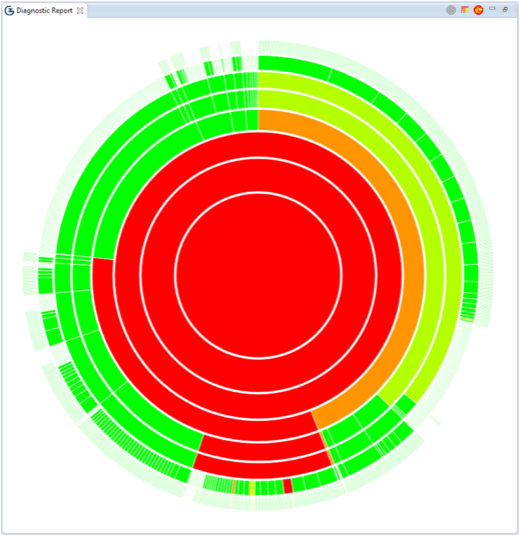
\includegraphics[width=0.5\textwidth]{barinel1.png}
    \caption{Visualização Sunburst do Crowbar}
    \label{fig:crowbar-sunburst}
  \end{center}
\end{figure}

Para além desta informação, a ferramenta apresenta-nos também com a lista de componentes ordenada de acordo com a probabilidade de este ter falhas.

% Software Repository Mining
\section{\emph{Software Repository Mining}}

\subsection{Identificação de correções e defeitos}

Na extração de informações de repositórios de código, como o \emph{Git}, torna-se importante identificar o tipo de alterações feitas. A descrição textual associada à alteração é bastante importante nesta identificação e permite fazê-lo com um elevado grau de precisão, dependendo do projeto em causa \cite{Mockus2000}.

É estimado que 34 a 46\% de todas as alterações correspondam a correções e que estas representem 18 a 27\% das linhas adicionadas e removidas \cite{Mockus2000}. Foram também encontrados padrões que relacionam as correções com o seu tamanho, em termos de código, e com o dia da semana em que foram executadas \cite{Sliwerski2005}.

Após esta identificação é possível identificar as alterações que introduziram os erros usando o algoritmo \emph{SZZ} \cite{Sliwerski2005}. Este algoritmo recorre ao histórico e à análise do código em questão para corretamente localizar o \emph{commit} (alteração) que introduziu o defeito, ignorando, por exemplo, alterações que apenas introduzam comentários.

\subsection{Ferramentas}

\subsubsection{\emph{libgit2}}

Libgit2\footnote{\url{https://libgit2.github.com/}} é uma biblioteca multi-plataforma, sem dependências, que permite a interação direta com o repositório \emph{Git} com uma performance nativa.

Esta biblioteca pode ser usada em qualquer linguagem que permita ligação a \emph{C}, pelo que existem dezenas de implementações em linguagem como \emph{Python}\footnote{pygit2 - \url{http://www.pygit2.org/}}, \emph{Javascript}\footnote{nodegit - \url{https://github.com/nodegit/nodegit}} e \emph{Java}\footnote{Jagged - \url{https://github.com/ethomson/jagged}}.

\subsubsection{\emph{GHTorrent}}

GHTorrent\footnote{\url{http://ghtorrent.org/}} é um projeto que tem por objetivo criar um armazém de dados escalável, facilmente pesquisável, mesmo \emph{offline}, que replique a informação obtida através da API REST do GitHub\footnote{\url{http://developer.github.com/}}.

Esta ferramenta funciona de uma forma distribuída e monitoriza a API do GitHub através da página \url{https://api.github.com/events}. Cada evento, despoleta a extração de informação e conteúdo para uma base de dados \emph{MongoDB} e outra \emph{MySQL} \cite{Gousios2012}.

% Abordagens à predição de defeitos
\section{Abordagens à previsão de defeitos}

Foram já exploradas algumas abordagens para a predição da qualidade do código. Salientam-se neste capítulo algumas técnicas como \emph{BugCache}, \emph{FixCache} e \emph{Buggy Change Classification}, que são técnicas que se incluem no tipo de abordagem que pretendemos seguir (\emph{change log}) e que permitem, em conjunto com outras técnicas, otimizar a localização dos defeitos.

\subsection{\emph{BugCache/FixCache}}

Com base na premissa de que as falhas nunca ocorrem isoladamente e que portanto onde existe um defeito existem outros, o \emph{BugCache} cria uma lista de componentes onde a probabilidade de conterem erros é elevada, com base na análise em todo o histórico de alterações do projeto.

Este algoritmo destaca-se pela sua precisão, conseguindo uma exatidão de 73 a 95\% quando usado com uma granularidade ao nível do ficheiro, sendo portanto o melhor até à data \cite{Kim2006}.

Os defeitos são identificados por ordem temporal e adicionados à lista. Quando esta lista atinge o tamanho máximo, os componentes vão sendo removidos de acordo com o método de substituição escolhido. Existem diversos métodos que utilizam diferentes métricas como última utilização (\emph{Least Recent Used - LRU}), número de defeitos recentes e número de alterações recentes \cite{Kim2006}.

Conclui-se com este algoritmo que \cite{Kim2006}:
%
\begin{itemize}
	\item Caso tenha sido introduzido um defeito, há uma tendência para serem introduzidos mais defeitos em breve. (\emph{temporal locality})
	\item Caso um componente tenha sido acrescentado ou modificado recentemente este tem uma maior probabilidade de ser defeituoso (\emph{changed-entity locality}, \emph{new-entity locality})
	\item Caso um componente tenha introduzido um erro, os componentes ligados mais diretamente a este introduzirão também erros no futuro (\emph{spatial locality})
\end{itemize}

A diferença entre o \emph{BugCache} e o \emph{FixCache} é o momento em que cada um atualiza a lista. Sendo que o primeiro atualiza a lista quando um defeito é introduzido, o segundo atualiza apenas quando o erro é corrigido. Devido a esta diferença a implementação do \emph{FixCache} torna-se mais fácil.

\subsection{\emph{Buggy Change Classification}}

\emph{Change Classification} tem uma abordagem fundamentalmente diferente e tem um objetivo também distinto. O \emph{Change Classification}, com recurso a técnicas de \emph{Machine Learning} e às informações disponíveis quanto a erros anteriores, é capaz de prever se uma alteração introduziu ou não um novo defeito. Esta previsão é feita com um rigor muito elevado de 78\% \cite{Whitehead2008}.

Numa primeira fase, todas as alterações feita até ao momento são classificados como \emph{buggy} ou \emph{clean}. Com esta classificação feita e com a extração de dados para cada também concluída, procede-se à criação de um modelo através do \"treino\" de um algoritmo de classificação.

O tipo de dados usados dividem-se em sete grupos: métricas de complexidade, código adicionado, código removido, nome do ficheiro e diretório, novo código e meta-dados \cite{Whitehead2008}.

Tanto \emph{Support Vector Machine} (SVM) como \emph{Naïve Bayes} foram usados no estudo, tendo sido o classificador feito com recurso a SVM aquele que apresentou melhores resultados \cite{Whitehead2008}.

% Machine Learning
% \section{\emph{Machine Learning}}

\subsection{\emph{Naïve Bayes}}

\subsection{\emph{Support Vector Machines} (SVM)}

\subsection{\emph{Random Forests}}


%Time-weighted Risk
%WhoseFault
%History slicing/Chronos
%SZZ